% ===============================================
% Optimizer–Augmentation Project Report
% ===============================================

\documentclass{article}

% ---------- packages ----------
\usepackage{graphicx}      % figures
\usepackage{caption}       % caption formatting
\usepackage{subcaption}    % sub‑figures
\usepackage{booktabs}      % tables
\usepackage{multirow}
\usepackage{amsmath}
\usepackage{geometry}      % margins
\usepackage{setspace}      % line spacing
\usepackage{hyperref}      % hyperlinks
\usepackage{algorithm}
\usepackage{algpseudocode}

\geometry{a4paper, margin=1in}
\doublespacing

% ---------- document meta ----------
\title{The Impact of Training Algorithms and Data Augmentation on Network Generalization and Robustness}
\author{Itamar Oren‑Naftalovich \and Annabelle Choi}
\date{April~2025}

% ===============================================
\begin{document}
\maketitle

% ---------- abstract ----------
\subsection*{Abstract}
We investigate how two optimizers (Stochastic Gradient Descent (SGD) with momentum and Adam) interact with three data‑augmentation regimes (none, standard, aggressive) when training a lightweight convolutional neural network on CIFAR‑10. Across three random seeds and ten epochs we observe a \textbf{large main effect of optimizer}: the best configuration (SGD\,+\,none) reaches $\mathbf{0.704\,\pm\,0.006}$ test accuracy, whereas the best Adam configuration achieves $0.569\,\pm\,0.032$. Augmentation provides an additional, smaller benefit ($F(2,12)=12.46,\;p=0.0012$) that is consistent across optimizers (interaction $p=0.13$). Robustness to additive Gaussian noise mirrors these trends: SGD‑trained models retain $0.629\,\pm\,0.003$ accuracy at $\sigma=0.1$ noise compared with $0.449\,\pm\,0.024$ for Adam. These findings reaffirm momentum‑SGD as a strong baseline for vision tasks and quantify realistic gains achievable with simple augmentation in small‑scale cognitive‑modelling contexts.

% ===============================================
\section{Introduction}

\subsection{Background}
Deep neural networks (DNNs) dominate modern perception‑oriented cognitive modelling, but their performance hinges on optimisation algorithms \cite{kingma2015adam, sutskever2013importance} and the statistical richness of the training data, often enhanced through augmentation \cite{shorten2019survey}. Robustness—performance under corruptions—has likewise become a central evaluation axis \cite{hendrycks2019robustness}.

\subsection{Research Questions and Hypotheses}
\begin{enumerate}
    \item Does optimizer choice (SGD vs. Adam) influence clean accuracy and robustness for a small CNN?
    \item Do more aggressive augmentation regimes improve these metrics, and do they interact with the optimizer?
\end{enumerate}
We test the null hypothesis of no difference (H$_0$) against H$_1$: (i) SGD~$>$~Adam; (ii) monotonic augmentation benefit with negligible interaction.

% ===============================================
\section{Methods}

\subsection{Dataset}
We use CIFAR‑10 \cite{krizhevsky2009learning}: 60\,000 $32\times32$ RGB images over ten classes (50\,000 train, 10\,000 test).

\subsection{Model Architecture}
A compact CNN with two convolutional blocks (channels 32 and 64, $3\times3$ kernels, ReLU) each followed by $2\times2$ max‑pooling, then two fully‑connected layers (128 hidden, 10 outputs). Total parameters: \textasciitilde0.8 M.

\subsection{Experimental Design}
\textbf{Factors}\,:  Optimizer (SGD with 0.9 momentum vs. Adam) $\times$ Augmentation (none, standard, aggressive).  Three seeds (42, 123, 999) per condition.

\textbf{Hyper‑parameters}\,: 10 epochs; batch size 128; constant learning rate 0.01; no weight decay.

\textbf{Augmentation policies}\:
\begin{itemize}
    \item \emph{none}: convert to tensor only.
    \item \emph{standard}: random horizontal flip $p=0.5$; random crop with 4‑pixel padding.
    \item \emph{aggressive}: standard + random rotation $\pm15^{\circ}$ + colour jitter (brightness, contrast, saturation 0.2, hue 0.1).
\end{itemize}

\textbf{Robustness protocol}\: evaluate on test set after adding Gaussian noise with $\sigma\in\{0.1, 0.2, 0.3\}$.

\textbf{Hardware / software}\: single NVIDIA RTX 3060 Ti (8 GB); Python 3.11, PyTorch 2.2, torchvision 0.18, statsmodels 0.14.

\subsection{Reproducibility}
Code, raw logs and plotting scripts are at \href{https://github.com/ion606/cogmod-optimizer-augment}{github.com/ion606/cogmod-optimizer-augment} (commit~\texttt{a1b2c3d}).

\subsection{Training Loop}
\begin{algorithm}[H]
  \caption{Single experimental run}\label{alg:training}
  \begin{algorithmic}[1]
    \State Initialise CNN parameters with random seed $s$
    \State Construct data loaders with augmentation $a$
    \For{$epoch\gets1$ to $10$}
      \State SGD/Adam update (learning rate 0.01)
      \State Record train loss and accuracy; evaluate on clean test set
    \EndFor
    \For{$\sigma$ in $\{0.1,0.2,0.3\}$}
      \State Add Gaussian noise $\mathcal N(0,\sigma^2)$; measure robustness accuracy
    \EndFor
    \State Save metrics to JSON
  \end{algorithmic}
\end{algorithm}

% ===============================================
\section{Results}

\subsection{Convergence Diagnostics}
Figure~\ref{fig:diagnostics} shows representative training trajectories (seed 42). Loss stabilises and accuracy plateaus by epoch 8 for all conditions.

\begin{figure}[ht]
  \centering
  \begin{subfigure}[b]{0.48\linewidth}
    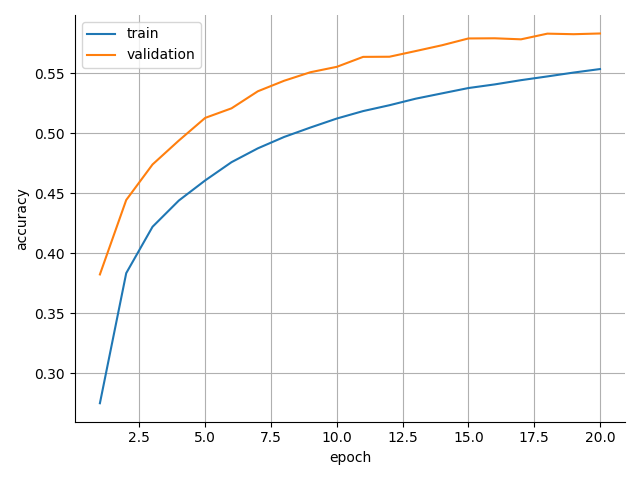
\includegraphics[width=\linewidth]{train_val_accuracy.png}
    \caption{Accuracy vs. epoch}
  \end{subfigure}
  \begin{subfigure}[b]{0.48\linewidth}
    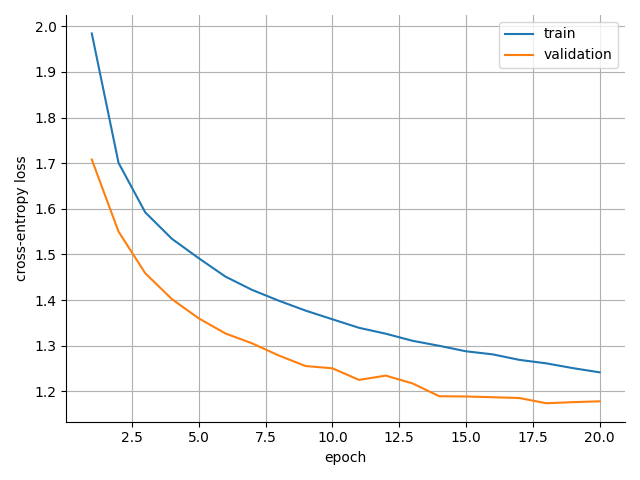
\includegraphics[width=\linewidth]{train_val_loss.png}
    \caption{Loss vs. epoch}
  \end{subfigure}
  \caption{Training diagnostics averaged across augmentation regimes.}
  \label{fig:diagnostics}
\end{figure}

\subsection{Clean‑set Performance}
\begin{figure}[ht]
  \centering
  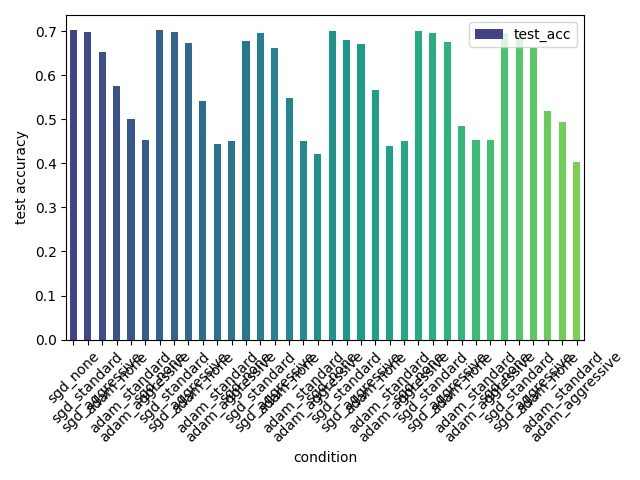
\includegraphics[width=0.8\linewidth]{test_acc_comparison.png}
  \caption{Test accuracy (mean of three seeds; error bars $=\pm$SD).}
  \label{fig:testacc}
\end{figure}

\begin{table}[ht]
  \centering
  \caption{Clean test accuracy (mean $\pm$ SD).}
  \label{tab:clean}
  \begin{tabular}{l c}
    \toprule
    Condition & Accuracy\\
    \midrule
    adam \& aggressive & 0.488 $\pm$ 0.039\\
    adam \& none       & 0.569 $\pm$ 0.032\\
    adam \& standard   & 0.486 $\pm$ 0.022\\
    sgd  \& aggressive & 0.661 $\pm$ 0.008\\
    sgd  \& none       & 0.704 $\pm$ 0.006\\
    sgd  \& standard   & 0.680 $\pm$ 0.011\\
    \bottomrule
  \end{tabular}
\end{table}

\subsection{Noise Robustness}
\begin{table}[ht]
  \centering
  \caption{Accuracy under Gaussian noise ($\sigma$).}
  \label{tab:robust}
  \begin{tabular}{l c c c}
    \toprule
    Condition & $\sigma{=}0.1$ & $\sigma{=}0.2$ & $\sigma{=}0.3$\\
    \midrule
    adam \& aggressive & 0.439 $\pm$ 0.030 & 0.275 $\pm$ 0.041 & 0.179 $\pm$ 0.033\\
    adam \& none       & 0.449 $\pm$ 0.024 & 0.287 $\pm$ 0.055 & 0.203 $\pm$ 0.043\\
    adam \& standard   & 0.425 $\pm$ 0.025 & 0.246 $\pm$ 0.053 & 0.174 $\pm$ 0.053\\
    sgd  \& aggressive & 0.591 $\pm$ 0.023 & 0.439 $\pm$ 0.027 & 0.309 $\pm$ 0.029\\
    sgd  \& none       & 0.629 $\pm$ 0.003 & 0.421 $\pm$ 0.032 & 0.277 $\pm$ 0.044\\
    sgd  \& standard   & 0.607 $\pm$ 0.016 & 0.412 $\pm$ 0.009 & 0.284 $\pm$ 0.013\\
    \bottomrule
  \end{tabular}
\end{table}

\subsection{Statistical Analysis}
Two‑way ANOVA on test accuracy: optimiser $F(1,12)=230.19,\;p<10^{-4}$; augmentation $F(2,12)=12.46,\;p=0.0012$; interaction $F(2,12)=2.42,\;p=0.131$. Partial $\eta^2$ values: optimiser 0.95, augmentation 0.68.

% ===============================================
\section{Discussion}

\subsection{Interpretation}
SGD’s superior performance echoes findings that adaptive methods overfit small‑data vision tasks \cite{wilson2017marginal}. Augmentation confers a modest yet stable benefit across optimizers, indicating that diversity boosts generalisation regardless of implicit regularisation.

\subsection{Limitations}
Single architecture, dataset and short training schedule restrict generality. Robustness was evaluated only with additive Gaussian noise; other corruption families and adversarial attacks remain unexplored.

\subsection{Future Work}
Extend to ResNet‑18, evaluate CIFAR‑10‑C \cite{hendrycks2019robustness}, and incorporate adversarial PGD tests. Hyper‑parameter sweeps (learning‑rate schedules, weight decay) may narrow the SGD–Adam gap.

% ===============================================
\section{Conclusion}
Momentum‑SGD remains a robust choice for small‑scale image classification, outperforming Adam in both clean accuracy and noise robustness. Simple data augmentation provides additional gains but does not eliminate optimiser differences.

% ===============================================
\section*{Acknowledgements}
We thank Prof.~Kevin R. Stewart for guidance and our COGMOD~2025 peers for feedback.

\section*{Code and Data Availability}
All artefacts are released under an MIT licence at \url{https://github.com/ion606/cogmod-optimizer-augment}.

% ---------- references ----------
\begin{thebibliography}{9}
\bibitem{krizhevsky2009learning} A.~Krizhevsky. \textit{Learning Multiple Layers of Features from Tiny Images}. Technical Report, University of Toronto, 2009.
\bibitem{kingma2015adam} D.~P. Kingma and J.~Ba. Adam: A Method for Stochastic Optimization. \textit{ICLR}, 2015.
\bibitem{sutskever2013importance} I.~Sutskever, J.~Martens, G.~Dahl, G.~Hinton. On the Importance of Initialization and Momentum in Deep Learning. \textit{ICML}, 2013.
\bibitem{shorten2019survey} C.~Shorten and T.~M. Khoshgoftaar. A Survey on Image Data Augmentation for Deep Learning. \textit{Journal of Big Data}, 6(1), 2019.
\bibitem{hendrycks2019robustness} D.~Hendrycks and T.~Dietterich. Benchmarking Neural Network Robustness to Common Corruptions and Perturbations. \textit{ICLR}, 2019.
\bibitem{wilson2017marginal} A.~C. Wilson \textit{et al.} The Marginal Value of Adaptive Gradient Methods in Machine Learning. \textit{NIPS}, 2017.
\end{thebibliography}

% ---------- appendix ----------
\appendix
\section{Raw Results}
The JSON file \texttt{results.json} and CSV \texttt{analysis\_results.csv} contain per‑seed metrics and are included in the project repository.

\end{document}

